\documentclass{article} 
% \usepackage[vietnamese]{babel}
\usepackage[utf8]{vietnam}
\usepackage{graphicx}
\usepackage{biblatex}
\bibliography{references.bib}

\graphicspath{{images/}}


\title{Báo Cáo về Phân Lớp Dữ Liệu Bằng Danh Sách Luật Bayesian cho Bài Toán Dự đoán Đột Quỵ}
\author{Nguyễn Hữu Lộc - 23C15031}
\date{31/12/2024}

\pagenumbering{arabic}

\begin{document}

\maketitle

\tableofcontents


\section{Giới thiệu sơ lược}
Với sự phát triển vượt trôi của các mô hình Large Language Model (LLM) trong thời gian gần đây, rất nhiều giải pháp đã được nghiên cứu và thử nghiệm nhằm mục đích tăng hiệu quả cho kết quả đầu ra, và giải quyết những vấn đề khó khăn. Đặc biệt quan tâm hơn cả là việc tính minh bạch của các mô hình LLM đang chịu nhiều chỉ trích do sự hình thành ảo giác trong quá trình suy luận, dẫn tới các phương pháp nhằm bổ sung dữ liệu cho mô hình Retrieval-Augmented Generation (RAG) được ra đời. Tuy nhiên các mô hình RAG lại có mặt hạn chế về cơ chế lấy dữ liệu từ các Cơ Sở Dữ Liệu Vector (CSDLV) một cách chưa thực tế và thường phụ thuộc vào cài đặt cố định, thiếu tính linh hoạt. Trong báo cáo này, nhóm sẽ giới thiệu đến một phương pháp mới có tính linh hoạt cao tên là Sel-Reflective Retrieval-Augmented Generation (Self-RAG) nhằm giải quyết vấn đề trên. Self-RAG sử dụng một mô hình tương tự như các mô hình LLM khác nhưng đã được huấn luyện lại cho phép nó có thể tự nhận xét, đánh giá câu trả lời thông qua các Reflection Token, được đưa vào bộ dữ liệu học nhằm mục đích cho phép mô hình tự đánh giá nếu câu trả lời có cần phải có trích dẫn hay không, và liệu trích dẫn hiện tại có phù hợp hay không. Từ đó, có 2 loại Reflection Token là "Retrieval" và "Critique" sẽ được đưa vào huấn luyện để mô hình tự tạo sinh ra, khác biệt so với các mô hình là truy cứu RAG rồi ghép vào prompt, còn Self-RAG sẽ tự tạo sinh ra lúc cần truy cứu. Đây chính là điểm tạo nên sự linh hoạt cho mô hình và giúp giảm chi phí huấn luyện. Chi tiết quy trình này có thể thấy thông qua phần bên phải của Hình \ref{fig:overview_self_rag}.

\begin{figure} 
    \centering
    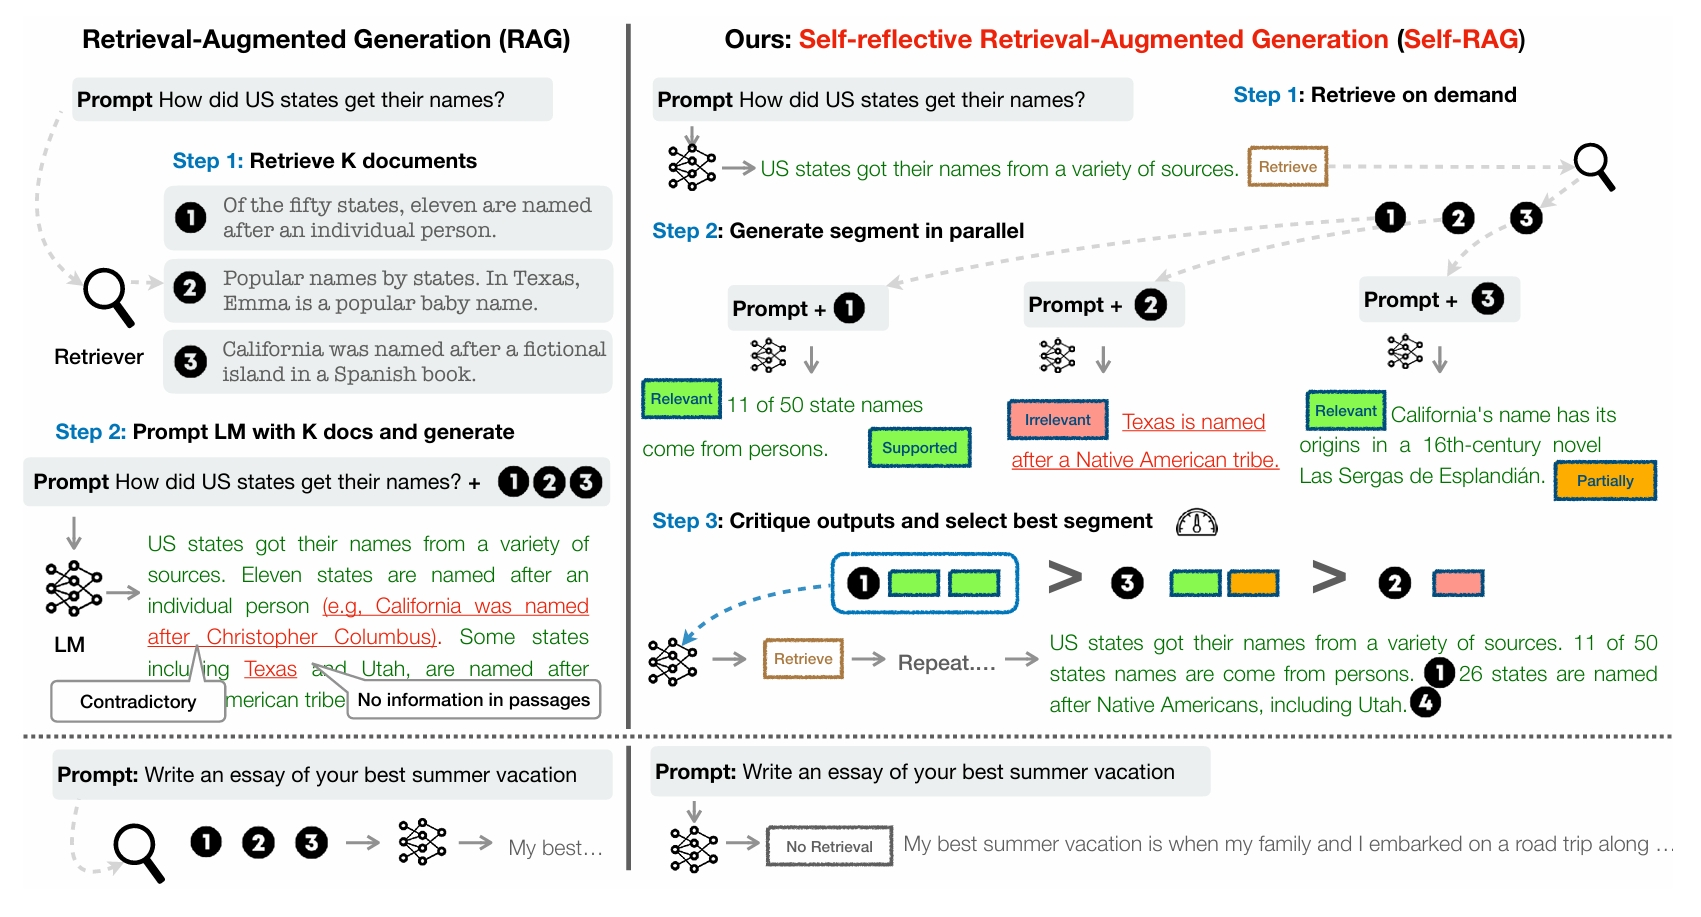
\includegraphics[scale = 0.2]{overview_self_rag.jpeg}
    \caption{Ví dụ về Danh Sách Luật Bayesian}
    \label{fig:overview_self_rag}
\end{figure}

Để chi tiết hơn thì quy trình của Self-RAG có thể được trình bày như sau: 

\begin{enumerate}
    \item Khi tiếp nhận prompts, mô hình đầu tiên sẽ suy luận nếu nó có cần phải truy cứu dữ liệu từ CSDLV hay không. Nếu cần, mô hình sẽ tạo sinh ra Reflection Token "Retrieval" và gọi truy cứu Retriver. 
    \item Kiểm tra xem các dữ liệu truy xuất ra từ CSDLV có tính liên quan với prompts input hay không và tạo sinh ra các câu trả lời tương ứng với từng dữ liệu. 
    \item Tạo sinh các token "Critique" và kiểm tra kết quả trả lời từ mô hình. Tiêu chí sẽ là tính đúng đắn (factuality) và chất lượng câu trả lời (overall quality) rồi cuối cùng mới trả lại câu prompts output.  
\end{enumerate}

Sự khác biệt của Self-RAG so với các mô hình RAG khác là ở chỗ mô hình sẽ tự tạo sinh ra Reflection Token và token này hình thành thông qua huấn luyện đặc biệt với bộ dữ liệu được xử lý bởi một mô hình "critic" khác. Dữ liệu huấn luyện cho Self-RAG đầu tiên sẽ được đưa qua mô hình "critic" để đánh giá, và thay thế các đoạn dữ liệu thành các Reflection Token "Retrieval" và "Critique" tương ứng, từ đó tạo nên bộ dữ liệu huấn luyện có sẵn những token này. Từ đó, dữ liệu này sẽ được đưa vào huấn luyện, cho phép Self-RAG có thể tự tạo ra những yêu cầu đánh giá và truy vấn theo nhu cầu. Điều này giúp tiết kiệm chi phí thay vì dùng 2 mô hình song song, 1 để tạo sinh câu trả lời và 1 để đánh giá, khi đưa vào thực tế như một vài phương pháp lồng ghép việc đánh giá kết quả từ truy vấn khác như mô hình Adaptive RAG \cite{jeong2024adaptive}. 

Việc sử dụng các Reflection Token cũng cho phép mô hình có sự linh hoạt cao hơn khi có thể cho phép người dùng tạo ra các giới hạn mềm, điều chỉnh số lượng truy vấn hoặc đánh giá theo nhu cầu. Điều này cải thiện được việc thiếu linh hoạt khi điều khiển cứng thông qua điều chỉnh tham số về số lượng truy vấn cho mỗi prompt input như các mô hình RAG ban đầu. 

Trong bài viết này cũng sẽ so sánh kết quả của mô hình với những mô hình phổ biến khác như ChatGPT3.0, Llama2-chat và Alpaca khi chỉ được trang bị cơ chế RAG phổ biến. Bên cạnh đó cũng chứng mình về tính hữu hiệu của việc ứng dụng Reflection token về mặt hiệu quả cả khi huấn luyện và khi suy luận của mô hình.  

\section{Các công trình liên quan}
Các nghiên cứu về RAG gần đây thiên hướng tìm cách để mô hình LLM có thể kết hợp dữ liệu truy xuất một cách nhuần nhuyễn hơn, hoặc tìm cách để tìm dữ liệu từ các CSDLV một cách chính xác, phù hợp hơn để phục vụ prompts input. Gần tương tự như Self-RAG, một vài mô hình cố gắng kết hợp việc truy xuất vào quá trình tạo sinh thay vì chỉ gọi truy xuất cố định vào ban đầu. Tuy nhiên những mô hình đó lại gặp vấn đề về chi phí tính toán và thiếu hiệu quả, dễ gặp vấn đề khi dữ liệu truy vấn thiếu liên quan do cơ chế không đủ linh hoạt, thích nghi kém. 

Một vài nghiên cứu thiên và hướng tinh chỉnh prompt trước khi đưa vào truy xuất nhằm tăng khả năng trả kết quả phù hợp thông qua fine-tune cho mô hình truy xuất và mô hình LLM. Một nghiên cứu dùng các phương pháp suy luận ngôn ngữ, và có mô hình dùng một mô hình tóm tắt (summarization model) để cô đọng thông tin và loại bỏ thông tin dư thừa cũng như tối ưu hóa trước khi đưa vào truy xuất. Dựa trên những ý tưởng trên nhưng hoàn thiện hơn thì Self-RAG cũng fine-tune dữ liệu huấn luyện để tăng khả năng truy xuất nhưng là thực hiện trực tiếp trên mô hình trong lúc suy luận, thay vì cần một mô hình phụ trợ khác. Và Reflection Token cũng giúp tinh gọn những thông tin dư thừa, giúp mô hình tập trung vào những thông tin quan trọng lúc truy xuất dữ liệu. 

Một hướng nghiên cứu khác đang có tính ứng dụng cao là fine tune các mô hình LLM thông qua việc sử dụng phản hồi của người (Reinforcement Learning from Human Feedback) để điều khiển các LLM trả lời, từ đó cho phép mô hình trả lời hiệu quả hơn. Tuy nhiên hướng đi này chủ yếu là giúp tinh chỉnh đầu ra của mô hình theo format mà người thiết kế muốn, hoặc điều chỉnh khả năng suy luận của mô hình hơn là tập trung vào việc trả lời một cách có trọng tâm và có dẫn chứng. Bên cạnh đó, Self-RAG do chỉ chỉnh sửa dữ liệu đầu vào trước khi đưa vào huấn luyện nên chi phí thấp hơn nhiều khi mà RLHF đòi hỏi cần có sự đánh giá của con người với các kết quả tạo sinh.


\section{Self-RAG: Học cách tìm nguồn, tạo sinh và đánh giá}

\subsection{Sơ lược bài toán và phương pháp}

\subsection{Huấn luyện Self-RAG}

\subsubsection{Huấn luyện phần đánh giá}

\subsubsection{Huấn luyện phần tạo sinh}

\subsubsection{Suy Luận}

\section{Thí nghiệm}

\subsection{Bài toán và dữ liệu}

\subsection{Cài đặt thí nghiệm}

\section{Kết quả và Phân tích} \label{sec:ketqua}

\subsection{Kết quả}

\subsection{Phân tích}

\section{Kết luận}


\printbibliography

\end{document}